\section{Modeling}
\label{sec:modeling}

In this section, we are going to introduce how we create the models fitting the best on the dataset to predict the Life.expectancy. The dataset that we used to after the data pre-processing and cleaning. The original dataset contains 157 observations and 23 variables in total to consider as the regression model. We removed X, Country, and Year from the original dataset and did some transformations to produce a better model in several steps for predicting the Life.expectancy in 2014 worldwide.

\subsection{Method overview}

In this subsection, we briefly introduce the methods that we used to complete the modeling. We used the multilinear regression, stepwise regression, user-defined variable transformation, and vif function as the Variance Inflation Factors in rstudio.

Multilinear regression is an extended regression of simple linear regression. It provides more functionalities so that it can support users to predict the response with multiple regressors. In R, the mlr function usually is used with the summary function to display the overall quality of the selected model. In the next few subsections, we will discuss how we implement the stepwise regression, variable transformation, and vif function in our model process.

Additionally, as the first regression model with all predictors, we got the Adjusted R-squared: 0.8615, F-statistic: 52.08 and p-value: $< 2.2\times 10^{-16}$ by executing the r code below:

\begin{verbatim}
summary(lm(Life.expectancy ~ ., data = Dat))
\end{verbatim}

According to the R output, not all regressors are significant enough to contribute to the prediction model. Thus, in the next steps, we tried to improve the Adjusted R-squared score with the knowledge that we learned in class STAT 5020.

\subsection{Data Transformation}

\begin{figure}
  \centering
  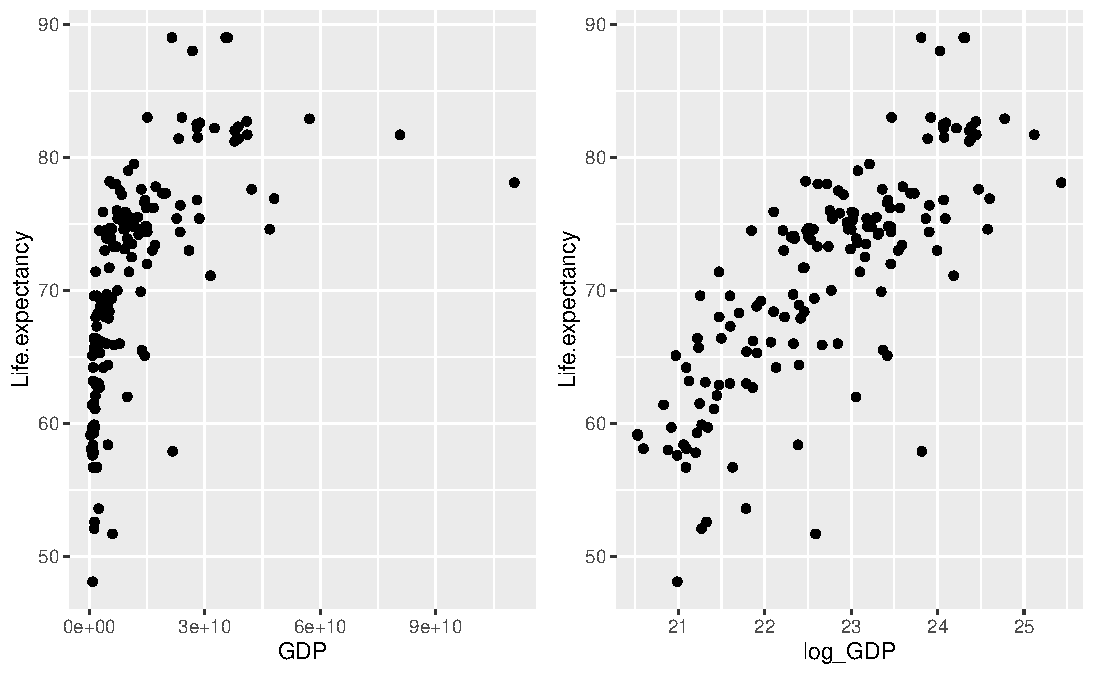
\includegraphics[width = 0.8\textwidth]{figures/transforms}
  \caption{Scatter plots of the GDP vs Life.expectancy variable before and after the transformation}
  \label{fig:transforms}
\end{figure}

In this subsection, the transformation that we applied to the dataset is described in detail. In figure \ref{fig:transforms} you can see GDP distribution before and after the log transformation. The transformation function is created as shown below:
\begin{verbatim}
transform <- function(x, scale) {
  if(scale == 0) return(log(1 + min(x) + x))
  else return(x^scale)
}
\end{verbatim}
The function takes two arguments, x as the original input value, and scale as the scaling value to be determined. We have a condition option for the user to choose when scale equals 0, the original input will be calculated as log(1 + min(x) + x); when the scale is given as a number that does not equal to 0, then the transformed input will be $x^{scale}$.



The dataset that we used in our project is after the transformation applied on log\_infant.deaths, log\_percentage.expenditure, log\_Measles, log\_under.five.deaths, log\_GDP, and log\_Population.

\begin{verbatim}
model2 <- lm(Life.expectancy ~ ., data = Dat2)
\end{verbatim}

Thus, we got the Adjusted R-squared: 0.8775, F-statistic: 59.83 and p-value: $< 2.2\times 10^{-16}$ from the new model with the new transformed dataset Dat2.

\subsection{Variance Inflation Factors}

The next step is to check the Variance Inflation Factors to check the collinearity problem, and this step is repeated several times as we finalize the model comparing with the correlation. We removed Hepatitis.B, log\_GDP, log\_Population, thinness.5.9.years, Income.composition.of.resources, and Schooling after the check. More details will be provided in the evaluation section.


\begin{verbatim}
Dat3 <- Dat2[,-c(7, 15, 16, 18, 19, 20)]
model3 <- lm(Life.expectancy ~ ., data = Dat3)
\end{verbatim}
The new model showed the Adjusted R-squared: 0.7849, F-statistic:  44.8, and p-value: $< 2.2\times 10^{-16}$.


\subsection{Stepwise modeling}

The stepwise model selection approach is a way to iteratively add and/or remove candidate variables to build a subset of variables in the provided dataset for a better model. Stepwise regression includes forward, backward, and bidirectional methods. In our project, we choose to use the bidirectional method for more flexible and appropriate models. The key r code to apply this step is listed below. Noted that as the column Status is a binary categorical field, we converted the text values to 1 for Developed and 0 for Developing.

\subsection{Bidirection model optimization}

\begin{verbatim}
DatSw <- Dat2
DatSw$Status <- ifelse(Dat$Status == "Developing", 0, 1)
stepwise(DatSw, "Life.expectancy", selection = "bidirection", select = "adjRsq")
\end{verbatim}

In the library(StepReg), stepwise is a built-in function that provides the functionalities for a user to choose the direction to select the predictors, as well as the criterion. "asjRsq" as adjusted r squared is used to judge if the model is good enough as the predictor selection process goes. During this step, variates "Adult.Mortality", "Alcohol", "log\_under.five.deaths", "HIV.AIDS","log\_percentage.expenditure", "Status", "Total.expenditure", "log\_infant.deaths", "Diphtheria", "BMI" and "thinness..1.19.years" are selected by the order of the improvement of "adjRsq".

\begin{verbatim}
DatSw <- select(Dat3_, c("Life.expectancy", sw$variate[-1]))
modelSw <- lm(Life.expectancy ~ ., data = DatSw)
\end{verbatim}

The model showed the Adjusted R-squared:  0.7876, F-statistic: 53.59 and p-value: $< 2.2\times 10^{-16}$. The adjusted R squared is expected to decrease since we now keep fewer variables in the current fitted model.

Then we choose to use vif function and remove the outliers later in the final model for optimization. Details will be provided separately in the Evaluation section. 

\subsection{Interactions}

% latex table generated in R 4.0.3 by xtable 1.8-4 package
% Thu Dec  9 18:45:49 2021
% latex table generated in R 4.0.3 by xtable 1.8-4 package
% Thu Dec  9 18:50:34 2021
% latex table generated in R 4.0.3 by xtable 1.8-4 package
% Thu Dec  9 18:51:17 2021
\begin{table}[ht]
\centering
\begin{tabular}{rlrr}
  \hline
 & v1v2 & $\Delta R^2$ & $\Delta adjR^2$ \\ 
  \hline
1 & Adult.Mortality*HIV.AIDS & 0.01650 & 0.01640 \\ 
  2 & Adult.Mortality*log\_under.five.deaths & 0.00680 & 0.00590 \\ 
  3 & Status*Diphtheria & 0.00680 & 0.00590 \\ 
  4 & Adult.Mortality*Total.expenditure & 0.00680 & 0.00580 \\ 
  5 & Adult.Mortality*log\_infant.deaths & 0.00660 & 0.00570 \\ 
   \hline
\end{tabular}
\caption{Effects of variable interaction} 
\label{tab:int}
\end{table}

Interactions are also a critical aspect that we wanted to consider. We have written a sinple R function, that acts like a forrward stepwise function. It probes all possible inteactions between two variables and takes the combination that produces the largest increase for the adjusted R2 metric. In table \ref{tab:int} you can see best 5 best variants and it is clear that  Adult.Mortality*HIV.AIDS one should be used to make our model more interpretable. As a result our final model is defined as
\begin{verbatim}
final_model <- lm(Life.expectancy ~ 
   Alcohol + log_percentage.expenditure + Status + Total.expenditure 
   + Adult.Mortality*HIV.AIDS, data <- DatSw)
\end{verbatim}

We got the Adjusted R-squared: 0.804 with the added interaction in the model, and after removing the variables that are not significant, we got Adjusted R-squared: 0.7959, F-statistic: 87.89 and p-value: $< 2.2\times 10^{-16}$. The outliers are taken care of in the last step and will be explained in the Evaluation section separately.
% The final model we got is shown below with the Adjusted R-squared 0.7959, F-statistic 87.89, and the p-value $< 2.2\time 10^{-16}$. We are satisfied with this model as it gives a good Adjusted R-squared as well as a relatively acceptable number of predictors in the model.

% \begin{verbatim}
% model_cleaned <- lm(
%   Life.expectancy ~  Alcohol + log_percentage.expenditure + Status +
%    Total.expenditure + Adult.Mortality*HIV.AIDS
% , data = Dat_cleaned)
% \end{verbatim}

%%% Local Variables:
%%% TeX-master: "main"
%%% End:
